% Для начала разберём, как базовый суперкомпилятор ведёт себя на
% базовом наборе программ, результат которых несложно проанализировать.

% \begin{itemize}
% \item Классическая программа \lstinline{doubleAppend}~\cite{cpd}, которая используется для
%       проверки наличия эффекта дефорестации (\todo{В приложении}).
% %\item Другая классическая программа \lstinline{maxLength}~\cite{cpd}, которая
% %      используется для проверки наличия эффекта таплинга.
% \end{itemize}

Разберём на примере результат работы базового суперкомпилятора.

Классическая программа для тестирования эффектов специализации ---
\lstinline{doubleAppend}, представленная на рисунке~\ref{fig:dappCode},
в которой происходит конкатенация списков трёх списков.

\begin{figure}[h!]
\begin{lstlisting}
doubleAppend a b c d =
  fresh (t)
   (append a b t $\land$ append t c d)
append y4 y5 y6 =
  (y4 $\equiv$ [] $\land$ y6 $\equiv$ y5) $\lor$
  fresh (ty t h)
   (y4 $\equiv$ h :: t $\land$
    y6 $\equiv$ h :: ty $\land$
    append t y5 ty)
\end{lstlisting}
\caption{Программа для тестирования \lstinline{doubleAppend}}
\label{fig:dappCode}
\end{figure}

Во многих бенчмарках~\cite{cpdPract, controlPoly} это программа используется
для проверки эффекта дефорестации.

Рассмотрим дерево процессов на рисунке~\ref{fig:dappTree}
(для компактности \lstinline{append} сокращён до \lstinline{app}),
которое порождается применением базового
суперкомпилятора к программе \lstinline{doubleAppend}, причём в
качестве аргументов --- простые свободные переменные, из-за чего
просто оптимизируется сама структура программы.

\begin{figure}[h!]
\center
\begin{minipage}[h]{\textwidth}
  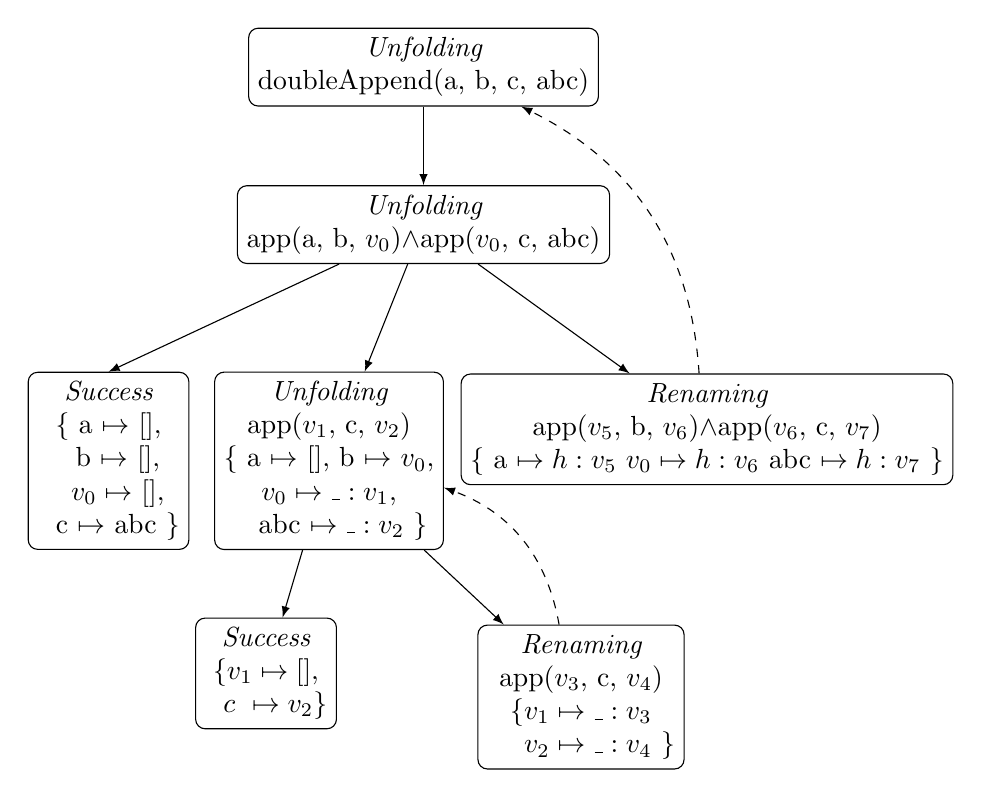
\begin{tikzpicture}[->,node distance=3cm, sibling distance=5cm, level distance=2cm]
    \tikzstyle{conf}=[rectangle,draw, rounded corners=.8ex,align=center]
    \node[conf] (root)   at (0, 0)     {{\it Unfolding} \\ \lstinline{doubleAppend(a, b, c, abc)}};
    \node[conf] (appapp) at (0, -2)    {{\it Unfolding} \\ \lstinline{app(a, b, $\text{v}_0$)$\land$app($\text{v}_0$, c, abc)}};
    \node[conf] (app1)   at (-1.2, -5) {{\it Unfolding} \\ \lstinline{app($\text{v}_1$, c, $\text{v}_2$)} \\ $\{$ a $\mapsto$ [], b $\mapsto$ $\text{v}_0$, \\ $\text{v}_0 \mapsto \_ : \text{v}_1$, \\ $\ \ $ abc $\mapsto \_ : \text{v}_2$ $\}$};
    \node[conf] (app2)   at (3.6, -4.6) {{\it Renaming} \\ \lstinline{app($\text{v}_5$, b, $\text{v}_6$)$\land$app($\text{v}_6$, c, $\text{v}_7$)} \\ $\{$ a $\mapsto \text{h} : \text{v}_5$  $\text{v}_0 \mapsto \text{h} : \text{v}_6 $  abc $\mapsto \text{h} : \text{v}_7$  $\}$};
    \node[conf] (appS)   at (-4,-5)    {{\it Success} \\ $\{$ a $\mapsto$ [], \\ \ \ b $\mapsto$ [],\\ \ \ $\text{v}_0 \mapsto$ [], \\ \ \ c $\mapsto$ abc $\}$};
    \node[conf] (app11)  at (2,  -8)  {{\it Renaming} \\ \lstinline{app($\text{v}_3$, c, $\text{v}_4$)} \\ $\{\text{v}_1 \mapsto \_ : \text{v}_3 $ \\ $\ \ \ \ \text{v}_2 \mapsto \_ : \text{v}_4 $  $\}$};
    \node[conf] (app1S)  at (-2, -7.7) {{\it Success} \\ $\{ \text{v}_1 \mapsto [],$ \\ $\ \ c \ \mapsto \text{v}_2 \}$};
    \draw[-latex] (root) -- (appapp);
    \draw[-latex] (appapp) -- (appS.north);
    \draw[-latex] (appapp) -- (app1);
    \draw[-latex] (appapp) -- (app2);
    \draw[-latex] (app1) -- (app1S);
    \draw[-latex] (app1) -- (app11);
    \draw[-latex,dashed] (app2) edge [bend right] (root);
    \draw[-latex,dashed] (app11) edge [bend right] (app1);
  \end{tikzpicture}
\end{minipage}
\caption{Дерево процессов для программы \lstinline{doubleAppend}}
\label{fig:dappTree}
\end{figure}

В приведённом дереве первым этапом происходит замена определения \lstinline{doubleAppend}
на его тело. Так как в определении нет дизъюнкий, получаем всего одну конфигурацию,
в которой операцией \lstinline{fresh} добавляется новая семантическая переменная $\texttt{v}_0$.
Далее происходит обработка конфигурации с более чем одним конъюнктом. Так как используется
полная стратегия развёртывания, каждая из конъюнкий раскрывается по определению и
рассматривается их дизъюнктивная нормальная форма, в которой всего четыре дизъюнкта,
один из которых не унифицируется, поэтому всего появляется только три конфигурации.
Эти конфигурации рассматривают несколько возможных значений переменных:
\begin{enumerate}
\item когда \lstinline{a} и \lstinline{b} пустые списки, то результатом конкатенации
является \lstinline{c};
\item если же \lstinline{b} не пуст, тогда результат --- это конкатенация списков \lstinline{b} и \lstinline{c}.
      Отношение конкатенации двух списков также специализируется под задачу.
      В результате этой специализации порождается исходное отношение, поскольку
      никакой новой информации не было выявлено и исходная программа уже была оптимальна;
\item в третьем же случае выводится, что результат конкатенации трёх списков
      \lstinline{a}, \lstinline{b} и \lstinline{c} --- это конкатенация
      списков $\texttt{v}_5$, \lstinline{b} и \lstinline{c}, где $\texttt{v}_5$
      является хвостом списка, а в голову которой добавили голову \lstinline{a}.
\end{enumerate}

По данному дереву порождается остаточная программа, изображённая на рисунке~\ref{fig:dappCodeOpt}.
\begin{figure}[h!]
\begin{lstlisting}
doubleAppendo a b c d =
  fresh (x4) (app3 a b x4 c d)
app3 a b t c d =
   fresh (x7 x6 x5 x10 x9 x8)
     (a $\equiv$ [] $\land$ b $\equiv$ t $\land$
       (t $\equiv$ [] $\land$ c $\equiv$ d $\lor$
       (t $\equiv$ x8 :: x9) $\land$
        d $\equiv$ x8 :: x10 $\land$
        app2 x9 c x10
     ) $\lor$
     (a $\equiv$ x5 :: x6 $\land$
      t $\equiv$ x5 :: x7 $\land$
      d $\equiv$ x5 :: x10 $\land$
      app3 x6 b x7 c x10) )
app2 a b c =
  fresh (x13 x12 x11)
   (a $\equiv$ [] $\land$ b $\equiv$ c $\lor$
   (a $\equiv$ x11 :: x12 $\land$
    c $\equiv$ x11 :: x13 $\land$
    app x12 b x13))
\end{lstlisting}
\caption{Суперкомпилированная программа \lstinline{doubleAppend}}
\label{fig:dappCodeOpt}
\end{figure}

В итоге, наблюдается, как двупроходный алгоритм становится однопроходным.
